\chapter{Soluciones coloidales} \label{chapter:mc:soluciones}
	
	\section{Introducci\'on}
	
	Los nanogeles son materiales que combinan las propiedades de los pol\'imeros y de los coloides. Son part\'iculas blandas, deformables y penetrables con una estructura formada por una red polim\'erica. \cite{lyon2012polymer} En soluci\'on, pueden absorber el solvente y encontrarse en un estado swelling \cite{karg2019nanogels,perez2021thermodynamic}
	La flexibilidad y la capacidad de responder a est\'imulos externos como la temperatura, la presi\'on, el pH, la fuerza i\'onica y la presencia de diferentes analitos, los convierten en objetos de inter\'es en diferentes aplicaciones tales como biosensores \cite{zhang2012ultrathin,islam2014responsive}, ingenier\'ia de tejidos \cite{matricardi2013interpenetrating,van2011biopolymer}, regeneraci\'on \'osea \cite{bai2018bioactive}, materiales biomim\'eticos \cite{green2016mimicking,wu2010multifunctional}, entre muchas otras aplicaciones biom\'edicas \cite{Daly2020}. 
	
	La capacidad de responder a diferentes est\'imulos externos viene mediada por la composici\'on de la red polim\'erica.
	Los nanogeles compuestos por cadenas de pol\'imero que contienen segmentos \'acidos como \'acido acr\'ilico o metacr\'ilico (AA y MAA, respectivamente) se expanden o comprimen  en respuesta a cambios en el pH de la soluci\'on \cite{snowden1996colloidal,Zhou1998}.
	De la misma forma, nanogeles compuestos pol\'imeros termosensibles experimentan una transici\'on de fase volum\'etrica cuando se calientan por encima de una temperatura caracter\'istica \cite{Pelton1986,Pelton2000}.
	Este comportamiento se origina porque estos pol\'imeros son insolubles en agua por encima de cierta temperatura cr\'itica m\'inima  de soluci\'on (LCST, por sus siglas en ingl\'es) \cite{Kawaguchi2020}.
	La incorporaci\'on de co-mon\'omeros termosensibles y con respuesta al pH, a la red polim\'erica,  permiten la obtenci\'on de nanogeles multi-responsivos los cuales son atractivos para el dise\~no de sistemas inteligentes que funciones en diferentes \'areas de la tecnolog\'ia \cite{plamper2017functional}.	
	
	Recientes avances en la s\'intesis han abierto el acceso a sistemas con arquitecturas y composiciones complejas, lo que permite adaptar estas part\'iculas con propiedades espec\'ificas. 
	Simult\'aneamente, enfoques te\'oricos y de simulaci\'on de vanguardia ofrecen una comprensi\'on m\'as profunda del comportamiento y la estructura de nanogeles y microgeles bajo influencias externas y confinamiento \cite{perez2021thermodynamic,scotti2022softness,urich2016swelling}. 
	Estudios te\'oricos sobre soluciones coloidales muestran a los nano/microgeles como part\'iculas esf\'ericas que interact\'uan \'unicamente con un potencial de n\'ucleo duro, es decir, esferas duras \cite{karg2019nanogels}. Encontr\'andose como variable termodin\'amica de relevancia la fracci\'on de volumen, lo que subraya la importancia de comprender y manipular estas interacciones en el dise\~no y aplicaci\'on de nanogeles y microgeles.
	Por otro lado \citet{alziyadi2023osmotic} utlizaron simulaciones de din\'amica molecuar con una teor\'ia de Posisson-Boltzmann para estudiar microgeles cargados superficialmente. En estos sistemas se incluyeron potenciales que permiten la deformaci\'on de los microgeles.
	En otros estudios, \cite{scotti2022softness,scheffold2020pathways}, se ha hecho \'enfasis en soluciones con concentraciones altas de microgeles, en las cuales  las part\'iculas se empaquetan densamente y forman una fase cristalina o amorfa. Esta capacidad de comprimirse y formar diferentes fases de los nano/microgeles se convierte en un aspecto clave que influye en las interacciones a nivel macrosc\'opica.
	La complejidad de la respuesta a est\'imulo de estas part\'iculas, a su vez, genera una mayor complejidad en cualquier dispersi\'on compuesta por ellas \cite{lyon2012polymer}. Las soluciones de nanogeles muestran un comportamiento mucho m\'as rico que el de sistemas modelados como esferas duras tradicionales y pueden ajustarse mediante cambios en las variables que afectan el tama\~no de las part\'iculas o la solvataci\'on.
	Las caracter\'isticas coloidales como las polim\'ericas de los nano/microgeles en dispersiones contribuyen a su fenomenolog\'ia.
	Estos dos aspectos complementarios de las suspensiones de microgeles ofrecen una amplia gama de posibilidades para su uso en el desarrollo de nuevas tecnolog\'ias. 
	Comprender la termodin\'amica de su respuesta a est\'imulo de estas soluciones se convierte en un estudio crucial.
	%%%%%%%%%
	
	En cap\'itulos anteriores se investig\'o la respuesta a est\'imulo de sistemas polim\'ericos aislados. En particular el cap\'itulo \ref{Chapter-geles} se dedic\'o al desarrollo de una teor\'ia termodin\'amica para el entendimiento de microgeles con respuesta a la temperatura, pH y concentraci\'on de sal. 
	En este nuevo cap\'itulo damos un paso m\'as adelante mostrando un estudio sistem\'atico de soluciones coloidales compuestos por nanogeles de poli-(N-isopropilacrialaminda) (P(NIPAm-co-MAA)). Para este prop\'osito se har\'a uso de una metodolog\'ia basada en algoritmos MonteCarlo en las cuales se combinan potenciales de interacci\'on part\'icula-part\'icula y un potencial termdin\'amico desarrollado en \cite{perez2021thermodynamic}. En este trabajo \citet{perez2021thermodynamic} describen la qu\'imica y f\'isica detr\'as de todos los fen\'omenos del swelling de sus microgeles impulsada por el pH, la dependencia no mon\'otona del tama\~no de part\'icula con la concentraci\'on de sal y el colapso de la red al aumentar la temperatura por encima de una temperatura caracter\'istica de transici\'on.
	Por otro lado los potenciales entre part\'iculas, Hertz-Yukawa, consideran la naturaleza de los nanogeles: su capacidad de deformarse, moderado por el potencial de Hertz y adquisici\'on de carga el\'ectrica, regulando la interacci\'on por el potencial de Yukawa.
	Se estudia la respuesta a est\'imulo de pH, temperatura, y concentraci\'on salina de nanogeles y como esta se ve modificada por la concentraci\'on de part\'iculas. 

	
	
	\section{Metodolog\'ia}
	
	Se realiz\'o un estudio sistem\'atico de la composici\'on de soluciones de nanogeles, variando la concentraci\'on salina, el pH y la concentraci\'on de part\'iculas. Adem\'as, se estudiaron estas soluciones a diversas temperaturas para observar el efecto de la temperatura sobre los mon\'omeros de NIPAm dentro de la red polim\'erica que compone a cada nanogel.
	
	\subsection{Potencial termodin\'amico intramolecular}
	
	La energ\'ia interna de cada nanogel se calcula en base al potencial termodin\'amico que tiene en cuenta toda la fisicoqu\'imica relevante del nanogel. En particular, se consideran la elasticidad de la red polim\'erica, la energ\'ia libre qu\'imica dada por los segmentos titulables (segmentos de MAA), la energ\'ia libre asociada a la entrop\'ia de mezcla de los iones que componen la soluci\'on, la energ\'ia por interacciones electrost\'aticas internas o con el solvente, as\'i como la energ\'ia generada por efectos est\'ericos.
	
	Para obtener este potencial termodin\'amico, es necesario considerar un modelo de dos fases. La primera fase est\'a ocupada por nuestro nanogel, cuya red polim\'erica esta compuesta por poli(NIPAm-co-MAA) (P(NIPAm-MAA)). Esta fase se denota por $NG$. La fase nanogel se encuentra en contacto con una soluci\'on acuosa (fase 2, denotada por $s$), en la cual estan presentes las mol\'eculas de agua, hidronio e hidr\'oxido, as\'i como tambi\'en los iones de prevenientes de la sal del medio.
	Con este modelo, podemos controlar variables externas como la temperatura $T$ y la composici\'on de la soluci\'on, es decir, el pH y la concentraci\'on de sal. Bajo estas condiciones, el nanogel asume un radio $R$ y, con ello, un volumen $V=\frac{4}{3}\pi R^3$.
	El potencial termodin\'amico cuyo m\'inimo produce las condiciones de equilibrio dentro de la fase de nanogel es un semi gran potencial, $\Omega_{NG}$.
	
	
	
	%
	\begin{align}
		\begin{aligned}
			\Omega_{NG}=& -TS_{mez} + F_{qca,MAA} +  F_{ela}\\
			& + U_{elec}+  U_{ste} + U_{VdW} -{\sum_{\gamma}
				{\mu_\gamma N_\gamma}}
		\end{aligned}
		\label{eq:mc:free-energy-implicit}
	\end{align}
	%
	
	
	\noindent En donde $S_{mez}$ es la entrop\'ia de traslaci\'on (y mezcla) de las especies libres en la fase del nanogel: mol\'eculas de agua ($w$), hidronio ($H_3O^+$) e iones de hidr\'oxido ($OH^-$), y cationes de sal ($+$) y aniones ($-$).
	Hemos considerado una sal monovalente, $KCl$,  completamente disociada en iones de potasio y cloruro.
	
	\begin{align}
		-\frac{S_{mez}}{k_B}	= \sum_{\gamma} \rho_\gamma\left(\ln\left(\rho_\gamma v_w\right) -1 + \beta\mu^0_\gamma\right) 
	\end{align}
	
	\noindent en donde  $\beta=\frac{1}{k_BT}$ , $T$ es la temperatura del sistema  y  $k_B$ es la constante de Boltzmann. La densidad num\'erica de la especie $\gamma$ es $\rho_\gamma$ y $\mu^0_\gamma$ es su potencial qu\'imico est\'andar,  $v_w$ es el volumen de una mol\'ecula de agua. Adem\'as $\gamma \in \left\{ w, H_3O^+, OH^-, +,- \right\}$.
	
	$F_{qca,MAA}$ es la energ\'ia qu\'imica libre que describe la protonaci\'on de equilibrio de las unidades de MAA.
	
	
	\begin{align}
		\beta F_{qca, MAA} =  \frac{\phi_{MAA}}{v_{MAA}} \left[f(\ln f+ \beta\mu^0_{MAA^-}) +(1-f)(\ln (1-f)+\beta\mu^0_{MAAH})\right]
	\end{align}
	
	
	\noindent donde $\phi_{MAA}$ es la fracci\'on de volumen que ocupan estos segmentos, siendo $v_{MAA}$ su volumen, y $f$ es el grado de disociaci\'on del mismo. 
	La fracci\'on de volumen de los segmentos MAA cargados es $f\phi_{MAA}$, y la de las unidades protonadas (o sin carga el\'ectrica) es $(1-f)\phi_{MAA}$.
	Los potenciales qu\'imicos est\'andar son $\mu^0_{MAA^-}$ y $\mu^0_{MAAH}$ para las especies desprotonadas (cargadas) y protonadas, respectivamente.
	Se define segmento como las unidades qu\'imicas que componen las cadenas de la red polim\'erica (MAA y NIPAm).
	
	
	La energ\'ia libre el\'astica que explica la libertad conformacional de la red polim\'erica es $F_{ela}$: 
	
	\begin{align}
		\beta F_{ela} = \dfrac{3}{2}\dfrac{N_{seg}}{n_{ch} }\left[\left(\dfrac{R}{R_0}\right)^2 - \ln\dfrac{R}{R_0} -1\right]
	\end{align}
	
	En donde $N_{seg}$ es el n\'umero total de segmentos en la red de pol\'imero y $n_{ch}$ es el n\'umero de segmentos por cadena de pol\'imero o \emph{longitud de cadena}.
	La constante de elasticidad en esta energ\'ia es proporcional al cociente $\dfrac{N_{seg}}{n_{ch}}$, que representa el n\'umero total de cadenas de pol\'imero en el nanogel.
	El radio del nanogel seco es $R_0$, lo que satisface:
	
	%
	%
	\begin{align}
		\begin{aligned} 
			\dfrac{4}{3}\pi R_0^3=V_0&=N_{seg}\Big( x_{MAA} v_{MAA} +x_{NIPAm} v_{NIPAm}\Big)
		\end{aligned}
	\end{align}
	
	
	\noindent donde $V_0$ es el volumen de la part\'icula seca; $x_{MAA}$ y $x_{NIPAm}$ son la fracci\'on de los segmentos MAA y NIPAm en el nanogel, respectivamente.
	El n\'umero total de segmentos MAA es $x_{MAA}N_{seg}$ y el de unidades NIPAm es $x_{NIPAm}N_{seg}$, estos \'ultimos con un volumen $v_{NIPAm}$.
	Los nanogeles que consideramos aqu\'i satisfacen $x_{NIPAm}=1-x_{MAA}$.
	
	
	$U_{elec}$ y $U_{ste}$ representan respectivamente las energ\'ias que resultan de las interacciones electrost\'aticas y las repulsiones est\'ericas.
	
	\begin{align}
		\beta U_{elec} =\left(\sum_{\gamma } {\rho_\gamma q_\gamma + f\dfrac{\phi_{MAA}}{v_{MAA}}q_{MAA}}\right)\beta\psi_{MG}
	\end{align}
	
	\noindent donde $q_\gamma$ y $q_{MAA}$ son la carga el\'ectrica de las moléculas $\gamma$ y de los segmentos de MAA, respectivamente.
	El potencial electrost\'atico dentro de la fase de nanogel es $\psi_{NG}$. Fuera de esta fase el potencial es nulo $\psi_s = 0$
	
	Se impone una restricci\'on de electro-neutralidad del microgel, que puede expresarse como:
	%
	%
	\begin{align}
		\begin{aligned}
			\sum_{\gamma  } \rho_\gamma q_\gamma + f\frac{\phi_{MAA}}{v_{MAA}}q_{MAA}=0
		\end{aligned}
		\label{eq:mc:charge-neutrality}
	\end{align}
	
	Las interacciones est\'ericas se incorporan como una segunda restricci\'on al sistema, la cual consiste en que el volumen de la fase nanogel est\'a completamente ocupado por los segmentos de la red y las especies qu\'imicas libres.
	
	%
	\begin{align}
		\begin{aligned}
			\sum_{\gamma } \rho_\gamma v_\gamma  + \phi_{MAA} + \phi_{NIPAm} = 1
		\end{aligned}
		\label{eq:mc:packing}
	\end{align}
	
	
	\noindent donde $v_\gamma$  es el volumen molecular de la especie $\gamma$, y la fracci\'on de volumen de cada componente de la red son: 
	%
	%
	\begin{align}
		\phi_{MAA}&=N_{seg}\dfrac{x_{MAA}v_{MAA}}{\frac{4}{3}\pi R^3}\\
		\phi_{NIPAm}&=N_{seg}\dfrac{x_{NIPAm}v_{NIPAm}}{\frac{4}{3}\pi R^3}
	\end{align}
	
	
	%%%%% 
	
	$U_{VdW}$ es la contribuci\'on que describe las interacciones efectivas pol\'imero-solvente; para este trabajo  se ha realizado la siguiente aproximaci\'on: 
	
	\begin{align}
		U_{VdW} = U_{NIPAm-w} + U_{MAA-w}
	\end{align}
	\noindent en donde $U_{NIPAm-w}$ incorpora la transici\'on hidrof\'ilica-hidrof\'obica de PNIPAm al aumentar la temperatura por encima de su temperatura de transici\'on cr\'itica. 
	Del mismo modo $U_{MAA-w}$ hace cuenta de la interacci\'on entre los segmentos de MAA y agua.
	Para el presente potencial intramolecular se ha considerado a los segmentos de MAA completamente hidrof\'ilicos y por tanto $U_{MAA-w} = 0$
	
	\begin{align}
		\beta U_{VdW} = U_{NIPAm-w} = \chi (T, \phi_{NIPAm})\rho_w \phi_{NIPAm}
	\end{align}
	
	
	Este  t\'ermino explica la respuesta de PNIPAm a los cambios de temperatura a trav\'es de un par\'ametro de interacci\'on pol\'imero solvente, $\chi$, que depende de la temperatura y la fracci\'on de volumen de NIPAm, $\phi_{NIPAm}$.
	Seg\'un  \citet{afroze2000}, este par\'ametro de Flory-Huggins se puede expresar como:
	%
	%
	
	
	\begin{align}
		\begin{aligned}
			\chi (T, \phi_{NIPAm}) &=g_0(T) +g_1(T)\phi_{NIPAm} \\
			&~+ g_2(T)\phi_{NIPAm}^2
		\end{aligned}
	\end{align}
	
	\noindent con
	%
	%
	\begin{align}
		\begin{aligned} 
			g_k(T)=g_{k0} + \frac{g_{k1}}{T} + g_{k2}T
		\end{aligned}
	\end{align}
	
	
	\noindent para  $k=0,1,2$, los coeficientes son: $g_{00}= -12.947$, $g_{02}=0.044959\,$K$^{-1}$, $g_{10}= 17.920$, $g_{12}= -0.056944$\,K$^{-1}$, $g_{20}= 14.814$, $g_{22}= -0.051419$\,K$^{-1}$  y $g_{k1}\equiv 0$ \cite{afroze2000}
	
	
	
	
	Finalmente, la suma sobre  $\gamma$ expresa el equilibrio qu\'imico con la fase de soluci\'on, donde $\mu_\gamma$ y $N_\gamma$ son el potencial qu\'imico y el n\'umero de mol\'eculas de la especie $\gamma$, respectivamente.
	%Aqu\'i, el subíndice $\gamma$ identifica  las especies qu\'imicas libres, $\gamma \in \left\{ w, H_3O^+, OH^-, +,- \right\}$.
	Hay que tener en cuenta que $\Omega_{NG}$ es un semi-gran potencial porque la fase del nanogel puede intercambiar cada una de estas mol\'eculas con la fase de soluci\'on, mientras que la red de pol\'imero est\'a confinada dentro de la primera.
	
	
	\begin{align}
		\sum_\gamma N_\gamma \mu_\gamma = \sum_{\gamma }{\rho_\gamma\beta\mu_\gamma}
		+ \beta\mu_{H^+}(1-f)\dfrac{\phi_{MAA}}{v_{MAA}}
	\end{align}
	
	Esta contribuci\'on muestra el equilibrio qu\'imico entre el nanogel y la fase de soluci\'on, donde el segundo t\'ermino en la derecha representa a los protones asociados a unidades de MAA;
	a saber, $\mu_{H^+}\equiv\mu_{H_3O^+}$ se conjuga con el n\'umero total de protones,
	
	\begin{align}
		N_{H_3O^+}+N_{MAAH}=V\left(\rho_{H_3O^+}+(1-f)\dfrac{\phi_{MAA}}{v_{MAA}}\right)
		\label{eq:mc:equilibrio}
	\end{align}
	
	
	
	Con todo esto la forma expl\'icita del potencial termodin\'amico es:
	
	
	
	
	%
	\begin{align}
		\begin{aligned}
			\beta&\frac{\Omega_{NG}(R)}{V}=\\& ~ \sum_{\gamma} \rho_\gamma\left(\ln\left(\rho_\gamma v_w\right) -1 + \beta\mu^0_\gamma\right) \\
			& + \frac{\phi_{MAA}}{v_{MAA}} \left[f(\ln f+ \beta\mu^0_{MAA^-})\right.\\
			&\qquad\left.+(1-f)(\ln (1-f)+\beta\mu^0_{MAAH})\right] \\
			%
			& + \dfrac{3}{2}\dfrac{N_{seg}}{n_{ch} V}\left[\left(\dfrac{R}{R_0}\right)^2 - \ln\dfrac{R}{R_0} -1\right] \\
			%
			& +  \left(\sum_{\gamma } {\rho_\gamma q_\gamma + f\dfrac{\phi_{MAA}}{v_{MAA}}q_{MAA}}\right)\beta\psi_{NG}\\
			%
			& +\beta\pi_{NG} \left[ \sum_{\gamma } \rho_\gamma v_\gamma  + \phi_{MAA} + \phi_{NIPAm} -1 \right] \\
			%
			& + \chi (T, \phi_{NIPAm})\rho_w \phi_{NIPAm} \\
			%
			& -\sum_{\gamma }{\rho_\gamma\beta\mu_\gamma}
			-\beta\mu_{H^+}(1-f)\dfrac{\phi_{MAA}}{v_{MAA}}\\
			%
			%
		\end{aligned}
		\label{eq:mc:free-energy}
	\end{align}
	
	
	
	
	\noindent En donde $\pi_{NG}$ es la presi\'on osm\'otica de la fase nanogel, introducido como un multiplicador de Lagrange para imponer la restricci\'on de incompresibilidad, ecuaci\'on \ref{eq:mc:packing}.
	
	
	Finalmente el potencial termodin\'amico esta escrito expl\'icitamente en funci\'on de las densidades de todas las especies, el grado de carga del MAA y el radio del nanogel, $\Omega_{NG}(R)\equiv\Omega_{NG}(\{\rho_\gamma\},f,R)$.
	Para obtener las expresiones de $\{\rho_\gamma\}$ y $f$ de tal forma que sean consistentes con el equilibrio termodin\'amico, minimizamos $\Omega_{NG}$ respecto a estas cantidades, y  sujeto a las restricciones ecuaciones  \ref{eq:mc:packing} y  \ref{eq:mc:charge-neutrality}; dicho procedimiento conduce a: 
	%
	%
	\begin{align}
		\rho_\gamma v_w &= a_\gamma \exp(-\beta\pi_{NG}v_\gamma -\beta\psi_{NG}q_{\gamma})\\
		\frac{f}{1-f}&= \frac{K^0_{MAA}}{a_{H^+}}\exp(-\beta\psi_{NG}q_{MAA})\label{eq:mc:fcharge}
	\end{align}
	
	\noindent donde $a_\gamma = e^{\beta\mu_\gamma-\beta\mu_\gamma^0}$ es la actividad de la especie $\gamma$. 
	La constante de equilibrio termodin\'amico que describe la protonaci\'on/desprotonaci\'on de los segmentos de MAA es:
	%
	%
	\begin{align}
		K^0_{MAA}= e^{\beta\mu^0_{MAAH}-\beta\mu^0_{MAA}-\beta\mu^0_{H^+}}
	\end{align}
	
	\noindent Esta cantidad es posible calcularla directamente a partir del pKa del \'acido.
	
	
	Si se considera  un valor de  $R$, las \'unicas inc\'ognitas restantes para determinar $\Omega_{NG}(R)$ son la presi\'on osm\'otica, $\pi_{NG}$ y el potencial electrost\'atico, $\psi_{NG}$.
	Estas dos cantidades se pueden calcular resolviendo num\'ericamente la incompresibilidad y la electro-neutralidad de la fase nanogel, ecuaci\'on \ref{eq:mc:packing} y ecuaci\'on \ref{eq:mc:charge-neutrality}, respectivamente.
	Para resolver estas ecuaciones utilizamos un m\'etodo h\'ibrido de Powell sin jacobiano y un c\'odigo FORTRAN desarrollado en el grupo de investigaci\'on.
	En resumen, es posible calcular la variaci\'on de  $\Omega_{NG}(R)$ en funci\'on del radio del nanogel $R$, y con ello calcular el valor del radio \'optimo del nanogel para unas condiciones dadas (pH, temperatura, concentraci\'on de sal).
	
	Una descripci\'on m\'as detallada del calculo del potencial termodin\'amico intramolecular puede encontrarse en la referencia  \cite{perez2021thermodynamic}
	
	\subsection{Energ\'ia intermolecular: Interacci\'on entre nanogeles.}\label{sec:mc:energia_intra}
	
	El segundo aporte energ\'etico que se considera en este trabajo es la interacci\'on de pares, es decir, la interacci\'on entre nanogeles dentro de la soluci\'on.
	Dadas las caracter\'isticas de nuestro sistema: part\'iculas blandas que pueden comprimirse/expandirse, as\'i como tambi\'en la capacidad de adquirir carga, se ha considerado un potencial combinado: Hertz-Yukawa.
	El primero cuantifica las interacciones el\'asticas efectivas entre cada par de part\'iculas. Permite la deformaci\'on de los nanogeles, cualidad intr\'inseca de nuestras part\'iculas.
	Por otro lado, el potencial de Yukawa se fundamenta en una teor\'ia de interacciones electrost\'aticas dependientes del medio en donde se encuentran.
	
	
	%%%%%%%% here
	
	Estos potenciales fueron previamente utilzados en \cite{weyer2018concentration}. \citet{weyer2018concentration} estudiaron la hinchaz\'on y las propiedades estructurales de suspensiones de microgeles i\'onicos.
	De forma expl\'icita se define el potencila de Yukawa como: 
	\begin{align}
		\beta u^Y_{ij}(r) = q_i q_j \frac{e^{\kappa(a_i + a_j)}}{(1 +\kappa a_i)(1 + \kappa a_j)} \frac{e^{-\kappa r}}{r} 
		\label{eq:mc:yukawa}
	\end{align}
	
	\noindent En donde $q_i$ y $q_j$ son las cargas netas que poseen los nanogeles $i$ y $j$ respectivamente. Del mismo modo se define el radio de cada part\'icula como $a_i$. El valor $\kappa$ corresponde a la constante de apantallamiento de Debye y $r$ es definido como la distancia entre los centros de masa de cada nanogel.
	
	El pontecial de Hertz  se define:
	\begin{align}
		\begin{aligned}
			& \beta u^H_{ij} (r) = \left(\frac{1-r}{a_i + a_j}\right)^{5/2}\times b_{ij} \\
			& b_{ij} = \frac{6}{5\pi}\frac{N_{chains}}{\frac{4}{3}\pi R_0^3}
		\end{aligned}
	\end{align}
	\noindent En donde $b_{ij}$ es la constante de interacci\'on entre la part\'icula $i$ y $j$ la cual tiene en cuanta el n\'umero de cadenas que compone al nanogel: $N_{chains}$, y el radio seco del mismo, $R_0$.
	
	Finalmente obtenemos:
	\begin{align}
		U_{inter}(r) = \begin{cases} U_H + U_Y & \text{if } r \leq a_i + a_j \\ U_Y & \text{if } r > a_i + a_j \end{cases} 
		\label{eq:mc:HY-potential}
	\end{align}
	
	\noindent en donde se define:
	
	\begin{align}
		& U_H = \sum^{Np}_{i \neq j} \beta u^H_{ij} \\
		& U_Y = \sum^{Np}_{i \neq j} \beta u^Y_{ij}
	\end{align}
	
	\noindent siendo $U_H$ y $U_Y$ la sumas sobre todos los pares de particulas $i$ $j$ que interactuan en la soluci\'on.
	
	
	
	\subsection{Metropolis-MonteCarlo}
	
	El modelado de las soluciones se realiz\'o utilizando el m\'etodo de Monte Carlo. Este se basa en la evaluaci\'on de diferentes estados o configuraciones del sistema de trabajo a trav\'es de la generaci\'on de n\'umeros aleatorios.
	En cada paso de la simulaci\'on, un estado del sistema es tomado y se intenta cambiar por una nueva configuraci\'on. Es decir, se pondera la probabilidad de que el sistema cambie a este nuevo estado. La ponderaci\'on de este cambio se realiza a trav\'es de la energ\'ia correspondiente al estado inicial y el estado nuevo al que se desea acceder.
	Este proceso se repite cierta cantidad de veces, este n\'umero es dependiente de la energ\'ia del sistema. Al finalizar, es posible obtener resultados estad\'isticamente significativos los cuales se utilizan para estimar propiedades macrosc\'opicas del sistema.
	En este cap\'itulo, se trata de una soluci\'on de nanogeles en el cual un cambio de configuraci\'on consiste en el movimiento y aumento/disminuci\'on de tama\~no de una part\'icula seleccionado al azar. Este esquema de trabajo puede visualizarse en la figura \ref{fig:mc:pasos_mc} en la cual se muestra un paso del algoritmo propuesto. Una part\'icula, en el estado \textbf{A}, de todas las presentes en la soluci\'on es cambiada de posici\'on, y en este caso, se disminuye su tama\~no, obteni\'endose el estado \textbf{B}.
	
	\begin{figure}[!htb]
		\centering
		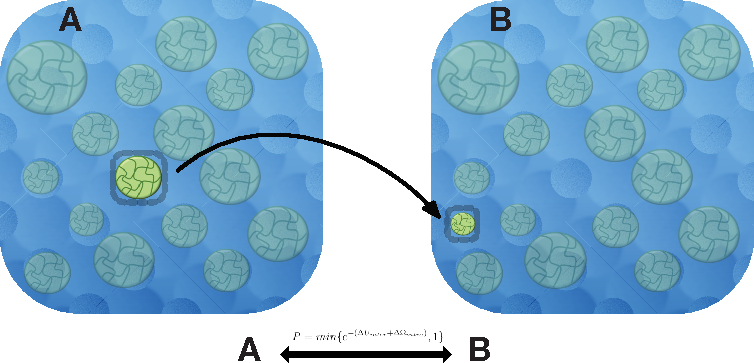
\includegraphics[width=0.65\textwidth]{Figures/modelos/mc_model.pdf}
		\caption{Esquema de un paso en el algoritmo de Metropolis-MonteCarlo. El paso de un estado \textbf{A} a uno \textbf{B} esta mediado por el cambio de energ\'ia entre ambas configuraciones. }
		\label{fig:mc:pasos_mc}
	\end{figure}
	
	
	
	
	La probabilidad de aceptar o no dichos cambios en el sistema viene dado por:
	
	\begin{align}
		P = min \{e^{-(\Delta U_{inter} + \Delta \Omega_{intra})},1\}
	\end{align}
	
	\noindent en donde $\Delta U_{inter}$ y $\Delta\Omega_{intra}$ son los cambios en energ\'ia de los estados inicial y final. De esta expresi\'on puede notarse que, si el cambio de energ\'ia es negativo, es decir, se pasa de un estado menos estable a uno energ\'eticamente m\'as estable, este paso es aceptado autom\'aticamente. S eobtiene una probabilidad de 1. 
	
	Si el cambio de energ\'ea es desfavorable, es decir, $\Delta U_{inter} + \Delta \Omega_{intra} > 0$, la probabilidad de aceptarlo es menor a uno. En este caso, se sortea un n\'umero aleatorio y, si este es menor o igual a la probabilidad de aceptaci\'on, el paso se acepta. De lo contrario, se rechaza. 
	
	
	\section{Nanogel aislado}
	
	En esta primera instancia caracterizamos a nuestro nanogel en dilusi\'on infinita. El calulo de su potencial termodin\'amico y como puede usarse para estudiar las fluctuaces en volumen de estos sistemas aislados.
	La respuesta a estimulo se estudi\'o es detallada en la referencia \cite{perez2021thermodynamic}. En donde adem\'as de ver los cambios en el pH, temperatua, y concentraci\'on de sal se estudia como son modificadas sus propiedades con la estructura del microgel.
	
	\subsection{Energ\'ia interna}
	
	En la figura \ref{fig:mc:energy-intra}, se observa el potencial termodin\'amico asociado a un nanogel aislado en funci\'on de su radio. Las curvas presentadas corresponden a tres concentraciones salinas. El pH del sistema es 4.65, el cual coincide con el pKa intr\'inseco del mon\'omero de MAA aislado. La temperatura para este sistema es de $25 ^\circ C$.
	El nanogel considerado en este estudio posee $N_{seg}=10^4$ segmentos con $n_{ch}=100$ segmentos por cadena, las cuales tienen un 35\% de MAA en su estructura polim\'erica, $x_{MAA}=0.35$. El 65\% restante est\'a compuesto por mon\'omeros de NIPAm.
	
	
	%El aumento de la concentraci\'on salina conlleva a un corrimiento del min\'imo energ\'etico hac\'ia valore m\'as grandes de radio. 
	
	
	\begin{figure}[!htb]
		\centering
		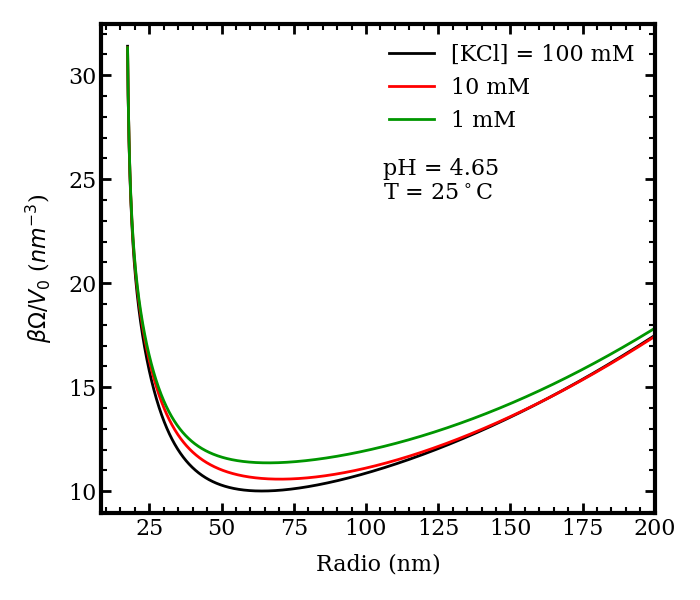
\includegraphics[width=0.45\textwidth]{Figures/graph-mc/interna.png}
		\caption{Energ\'ia libre de un nanogel aislado en funci\'on del tama\~no del mismo. Las curvas corresponden a diferentes condiciones de pH. La concentraci\'on salina es 1 mM y la temperatura $25 ^\circ C$.}
		\label{fig:mc:energy-intra}
	\end{figure}
	
	
	
	
	\subsection{Fluctuaci\'on en Volumen}\label{sec:mc:fluctuacion}
	
	Las fluctuaciones en volumen son la variaci\'on aleatoria del volumen de un sistema. En esta instancia, se muestran las fluctuaciones en volumen esperadas para un sistema aislado. Estas fluctuaciones son de gran utilidad dado que pueden ser extrapolables a soluciones m\'as concentradas.
	La fluctuaci\'on en volumen es una medida de la inestabilidad del volumen de un sistema termodin\'amico. A mayor fluctuaci\'on, mayor es la inestabilidad.
	La f\'ormula para la fluctuaci\'on en volumen de un sistema termodin\'amico se ha descrito como:
	
	\begin{align}
		\frac{\Delta V}{V} = \sqrt{\frac{k_BT}{V}\kappa_T}
	\end{align}
	
	\noindent en donde $\Delta V$ es la fluctuaci\'on en volumen, $V$ es el volumen del sistema, $k_B$ es la constante de Boltzmann, $T$ es la temperatura del sistema y $\kappa_T$ es la constante de incompresibilidad isot\'ermica. 
	
	La constante de compresibilidad isot\'ermica, $\kappa_T$, es una medida de la rigidez del sistema. A mayor $\kappa_T$, mayor rigidez del sistema.
	Se define como la relación entre la variaci\'on de presi\'on y  volumen de un fluido a temperatura constante, considerando nuestro potencial termodin\'amico, $\Omega_{NG}$, se puede obtener la siguiente forma:
	
	
	\begin{align}
		\begin{aligned}
			\kappa_T & = -\frac{1}{V} \left( \frac{\partial V}{\partial P}\right)_T \\
			& =\frac{1}{V} \left( \frac{\partial^2 \Omega_{NG}}{\partial V^2}\right)^{-1}_T \\
			& = 12 \pi R_{eq} \left( \frac{\partial^2 \Omega_{NG}}{\partial R^2}\right)^{-1}_{T,R=R_{eq}}
		\end{aligned}
	\end{align}
	\noindent en la cual $R_{eq}$ hace referncia al radio de equilibrio, es decir al m\'inimo de las curvas de la energ\'ia $ \Omega$, presentadas en \ref{fig:mc:energy-intra}. Todas las dem\'as variables fueron previamente definidas en la secc\'ion \ref{sec:mc:energia_intra}
	
	\begin{figure}
		\centering
		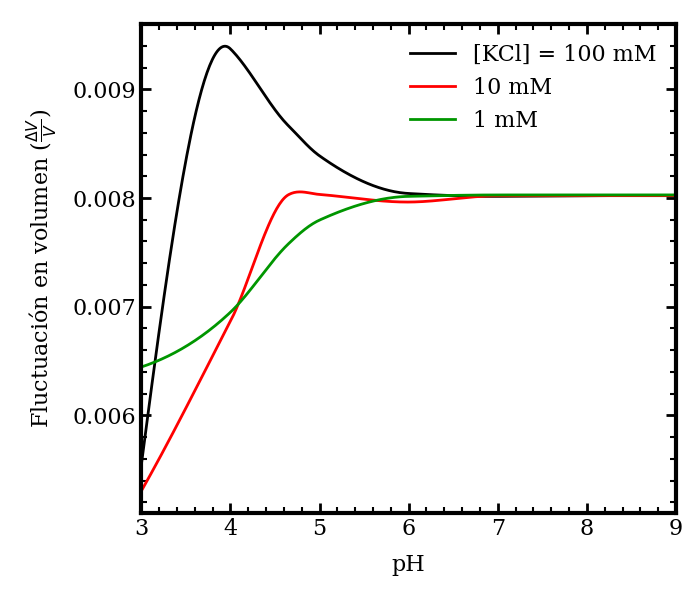
\includegraphics[width=0.45\linewidth]{Figures/graph-mc/fluct-pH.png}
		\caption{Gr\'afico de la fluctuaci\'on en volumen de un nanogel aislado. El nanogel esta compuesto por $2\times 10^5$ segmentos (mon\'omeros) repartidos en 200 cadenas de 1000 cadenas cada una}
		\label{fig:mc:flut-pH}
	\end{figure}
	
	En base a estas consideraciones, se confeccion\'o la figura \ref{fig:mc:flut-pH}. En esta figura, se observa la fluctuaci\'on en tama\~no de un nanogel aislado en funci\'on del pH del bulk de la soluci\'on. Se presentan curvas correspondientes a tres condiciones salinas: 1, 10 y 100 mM en KCl. La temperatura es de 25$^\circ$C, condiciones en las cuales el PNIPAm posee un comportamiento hidrof\'ilico. En estas condiciones, las fluctuaciones mostradas en esta figura no se ven afectadas por la presencia de este co-mon\'omero.
	
	En t\'erminos generales, se observa que la fluctuaci\'on del sistema a las diferentes condiciones presentadas es de muy baja magnitud, del orden de $10^{-3}$. Sin embargo, dentro de estos valores, se puede notar un aumento de la fluctuaci\'on al aumentar el pH hasta estabilizarse en valores de pH mayores a 6.
	
	A bajos valores de pH, el nanogel no posee carga, ya que los mon\'omeros de MAA que componen la red polim\'erica se encuentran desprotonados (estamos por debajo del pKa intr\'inseco del MAA). En estas condiciones, un cambio en el tama\~no del nanogel conlleva cambios en la energ\'ia dada por la adsorci\'on de solvente y de los iones presentes en el sistema, adem\'as de la contribuci\'on el\'astica que conlleva el cambio de radio.
	La entrada o salida de iones conlleva un cambio en la cantidad de carga dentro del nanogel, con lo cual se esperar\'ia un aumento en el grado de carga de los mon\'omeros. Sin embargo, estas condiciones son desfavorables para bajos valores de pH, por lo que las fluctuaciones son las m\'as bajas en estas condiciones.
	En particular, altas concentraciones salinas promueven una desprotonaci\'on de los segmentos de MAA para peque\~nos aumentos de pH. Esto se debe a que los iones presentes en la soluci\'on pueden apantallar la carga el\'ectrica adquirida por los grupos carbox\'ilicos de los mon\'omeros de MAA. Como resultado, la entrada de iones favorece la fluctuaci\'on en volumen del nanogel.
	A medida que aumenta el pH, m\'as unidades de MAA adquieren carga el\'ectrica, por lo cual un cambio en su volumen se ve favorecido. Para minimizar las repulsiones el\'ectricas de la red polim\'erica, el nanogel puede expandirse o adsorber m\'as cantidad de contraiones presentes en la soluci\'on. Como resultado, se observa un aumento en la fluctuaci\'on del sistema, el cual se intensifica con el aumento de la concentraci\'on salina.
	
	A condiciones de pH altos, el nanogel se encuentra completamente desprotonado, cargado el\'ectricamente. La salida o entrada de iones, que podr\'ia provocar un cambio en la carga del nanogel, es m\'as favorable que a bajos pH. Por ello, se observa una fluctuaci\'on mayor, pero menor que a valores intermedios de pH, en los que la desprotonaci\'on es incompleta y el nanogel puede expandirse o contraerse. En cambio, a condiciones de pH alto solo es posible una expansi\'on del nanogel, ya que no hay efecto de los contraiones de sal.
	
	
	
	%%%%%%%%%%%%%%%%%%%%%%%%%%%
	
	En la figura \ref{fig:mc:fluct-T} se muestra el efecto de la temperatura en las fluctuaciones en el volumen del nanogel. Se presentan tres curvas correspondientes a tres valores caracter\'isticos de pH: por debajo y por encima del pH intr\'inseco del MAA, pH 3 y 7, respectivamente, y una al valor del pKa del MAA aislado, 4.65.
	Para el pH 3, el grado de carga el\'ectrica del nanogel es pr\'acticamente nulo, por lo cual las fluctuaciones que se observan son por efecto de la temperatura. Bajo este pH, se ve que no hay cambios apreciables a medida que se aumenta la temperatura del sistema. El nanogel es estable a todas las temperaturas de trabajo, incluso cerca de la temperatura de transici\'on del PNIPAm, alrededor de los 32$^\circ$C. En este punto, el nanogel adopta un estado colapsado y no hay ninguna fuerza impulsora que promueva un peque\~no cambio en su volumen.
	%%%%%%%%%
	
	A pH 4.65 y 7, el sistema posee carga el\'ectrica. Por tanto, al agregarle energ\'ia al sistema (aumento de temperatura), las fluctuaciones aumentan. Esto ocurre hasta llegar a la temperatura caracter\'istica de transici\'on volum\'etrica del PNIPAm. Despu\'es de este punto, hay un colapso en la estructura del nanogel, siendo las interacciones entre los segmentos de NIPAm las predominantes y estabilizando un tama\~no espec\'ifico del nanogel.
	La probabilidad de que se d\'e un cambio en el volumen es muy baja y, por tanto, se observa un decaimiento de las fluctuaciones.
	En particular, las fluctuaciones son mayores a pH 4.65 dado que el nanogel posee menor proporci\'on de segmentos de MAA cargados. A pH 7, todos est\'an completamente cargados. a pH 4.65 se permite un equilibrio entre segmentos protonados/desprotonados con la entrada de contraiones de sal y, de esta forma, permitir una expansi\'on/contracci\'on del nanogel.
	
	
	
	\begin{figure}
		\centering
		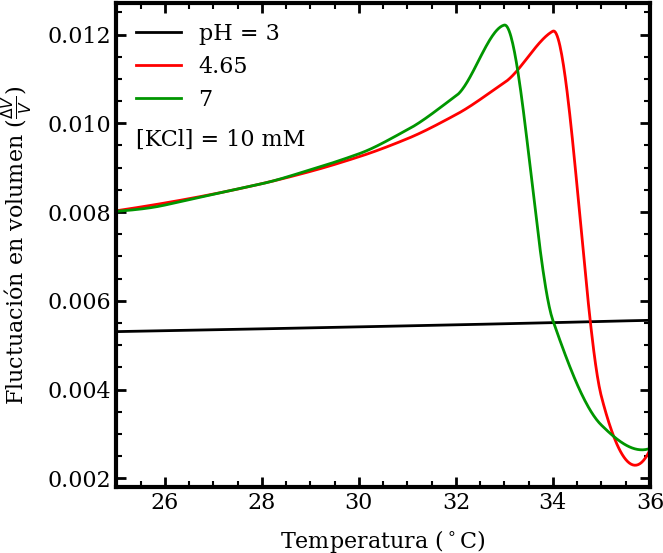
\includegraphics[width=0.45\linewidth]{Figures/graph-mc/fluct-T.png}
		\caption{Gr\'afico de la fluctuaci\'on en volumen de un nanogel aislado. El nanogel esta compuesto por $2\times 10^5$ segmentos (mon\'omeros) repartidos en 200 cadenas de 1000 cadenas cada una}
		\label{fig:mc:fluct-T}
	\end{figure}
	
	
	\section{Resultados}
	
	En esta secci\'on mostraremos los resultados obtenidos en el estudio sistem\'atico de soluciones de nanogeles compuestos por segmentos de N-isopropilamina (NIPAm) y \'acido metacr\'ilico (MAA). La red polim\'erica, P(NIPAm-co-MAA), posee un 35\% de MAA.
	A cada una de estas soluciones se estudiaron su respuesta a cambios en el pH, la temperatura y la concentraci\'on salina. En cada caso se comparar\'a con un nanogel a diluci\'on infinita, es decir, un sistema aislado.
	
	
	\subsection{Simulaciones Montecarlo}
	
	En esta secci\'on mostraremos los resultados de las simulaciones Monte Carlo. Estas se componen de  $5\times 10^6$ pasos, cada paso de simulaci\'on se compone de una compresi\'on/expansi\'on y cambio de posici\'on espacial de una part\'icula que compone la soluci\'on. La caja de simulaci\'on est\'a compuesta por 500 nanogeles.
	
	En la secci\'on anterior, secci\'on \ref{sec:mc:fluctuacion}, se menciona que las fluctuaciones de un nanogel aislado son peque\~nas, por lo que en principio se esperar\'ian cambios peque\~nos en una distribuci\'on de tama\~nos. Sin embargo, al considerar estas part\'iculas en soluci\'on se pone en juego una nueva contribuci\'on energ\'etica: interacciones interparticulares. Estas vienen reguladas por los potenciales presentados en la ecuaci\'on \ref{eq:mc:HY-potential}.
	Estos nuevos potenciales proporcionan al sistema la capacidad de aumentar las fluctuaciones en tama\~no de los nanogeles. %Mostraremos esto en los resultados a continuaci\'on.
	
	%%%%
	En la figura \ref{fig:mc:densidad-probabilidad} se muestra la densidad de probabilidad de distribuci\'on de tama\~nos de tres soluciones de nanogeles. Las condiciones del bulk de la soluci\'on son pH 4.76, temperatura 25$^\circ$C y una concentraci\'on de sal de 1 mM en $[KCl]$.
	Cada curva representa una diferente fracci\'on en volumen y/o diferente factor de empaquetamiento. Este factor se define como:
	
	
	
	\begin{align}
		\zeta = \frac{4}{3} \pi r^3 N_p \frac{1}{V}
	\end{align}
	
	En donde V corresponde al volumen de la caja de simulación, $N_p$ el n\'umero de part\'iculas de la soluci\'on y $r$ es un valor de referencia.
	Para todas las simulaciones se ha considerado $r= 2D_0$, en donde $D_0$ es el di\'ametro de un nanogel seco. Es decir, solo se considera el volumen molecular de todos los segmentos que lo componen.
	Con un n\'umero de part\'iculas y el valor de $r$ fijos, sabemos que un valor de $\zeta$ grande corresponde a un volumen m\'as peque\~no. Es decir, una soluci\'on m\'as concentrada.
	De forma similar, para un $\zeta$ peque\~no obtenemos una soluci\'on m\'as diluida.
	
	\begin{figure}
		\centering
		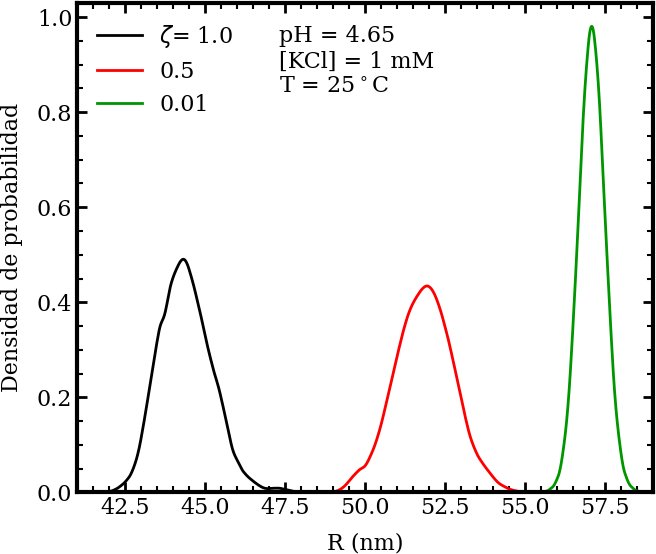
\includegraphics[width=0.45\linewidth]{Figures/graph-mc/size-zetas.png}
		\caption{Densidad de probabilidad de tama\~no para 3 diferentes soluciones. Se considera un factor de empaquetamiento de $\zeta$ = 1.0, 0.5 y 0.01 para cada una de las soluciones. El radio de un nanogel aislado es de 57.2 nm. Las condiciones bulk para el potencial intramolecular, $\Omega_{NG}$, corresponden a pH 4.65, temperatura 25$^\circ$C y 1 mM en [KCl].}
		\label{fig:mc:densidad-probabilidad}
	\end{figure}
	
	Se puede observar en la figura \ref{fig:mc:densidad-probabilidad} que a soluciones m\'as concentradas hay una mayor dispersi\'on en los tama\~nos de cada part\'icula. La cercan\'ia de las part\'iculas en estas soluciones permite que interact\'uen m\'as poni\'endose en juego una mayor variabilidad de tama\~nos que logren minimizar la energ\'a del sistema.
	Para las soluciones diluidas, $\zeta =$ 0.01, los nanogeles tienden a estabilizarse a un \'unico valor de radio. La baja probabilidad de interacci\'on entre part\'iculas resulta en un sistema aislado y, por tanto, la fluctuaci\'on en su volumen ser\'a menor.
	Tambi\'en en esta soluci\'on m\'as diluida vemos que el m\'aximo de la distribuci\'on tienda al radio de m\'inima energ\'ia dado en la curva \ref{fig:mc:energy-intra} a concentración de 1 mM en  $[KCl]$. Es decir, se tiende a un sistema aislado.
	
	%%%%%%%
	En la tabla \ref{tabla:mc:R-optimos} se muestran los valores de $R$ correspondientes al pico m\'aximo de probabilidad. Se observa que a mayor concentraci\'on de nanogeles, su radio medio disminuye, y a medida que diluimos m\'as la soluci\'on, el radio medio se acerca al radio que minimiza el potencial termodin\'amico de un nanogel aislado.
	Esta disminuci\'on del tama\~no puede explicarse al considerar los potenciales de interacci\'on entre part\'iculas. Al estar las part\'iculas muy pr\'oximas entre s\'i, interact\'uan bajo la influencia de los potenciales de Hertz-Yukawa. Para disminuir la energ\'ia dada por estas interacciones, los nanogeles buscan disminuir su tama\~no, si bien esto conlleva un aumento en la energ\'ia libre interna del nanogel, ver figura \ref{fig:mc:energy-intra}, este aumento es costosamente menor que el originado por los potenciales de Hertz-Yukawa.
	
	A medida que disminuimos la concentraci\'on de nanogeles, estos pueden aumentar su tama\~no para acercarse m\'as a su radio ideal. Es por ello que en ausencia de interacciones de a pares, una diluci\'on infinita, las part\'iculas tienen a aumentar su radio hasta minimizar la energ\'ia interna.
	
	
	\begin{table}[!htb]
		\centering
		\begin{tabular}{|c|c|} \hline  
			$\zeta$& $R_0$ (nm)\\ \hline  
			1.0& 44.5\\ \hline  
			0.5& 52.0\\ \hline  
			0.01& 57.1\\ \hline
			Aislado & 57.2 \\ \hline
		\end{tabular}
		\caption{Tabla con los valores de radio \'optimo para las condiciones bulk de pH = 4.65, temperatura = 25$^\circ$C, y [KCl] = 1 mM.}
		\label{tabla:mc:R-optimos}
	\end{table}
	%%%%
	
	Los resultados monstrados con anterioridad muestran que la capacidad de fluctuaci\'on de tama\~no de los nanogeles es fuertemente afectada por su capacidad de interactuar con otro nanogel vecino, lo cual est\'a influenciado por la concentraci\'on de la soluci\'on.
	En ese sentido, la figura \ref{fig:mc:rdf} muestra la densidad de distribuci\'on radial para las tres diferentes soluciones de nanogeles. Consideramos las mismas condiciones del bulk de la figura \ref{fig:mc:densidad-probabilidad}, es decir, pH 4.65, temperatura de 25$^\circ$C y concentraci\'on salina 1 mM.
	En el inset se muestra la solución con $\zeta =$ 0.01.
	Se puede observar que los perfiles para las soluciones m\'as concentradas corresponden al comportamiento de un sistema l\'iquido. Para estos casos, $\zeta = $ 1.0 y 0.5, notamos un primer pico correspondiente a los primeros vecinos. Este primer m\'aximo se encuentra a una distancia aproximada del di\'ametro de un nanogel de equilibrio, en esas condiciones de bulk de soluci\'on. Ver tabla \ref{tabla:mc:R-optimos}.
	
	Los siguientes m\'aximos observables hacen referencia a la segunda capa de ``hidrataci\'on'' a mayor distancia y una menor magnitud respecto de la primera.
	Para el sistema m\'as diluido, $\zeta =$ 0.01, su comportamiento se asemeja m\'as a un sistema gaseoso, en la cual la distribuci\'on radial es uniforme y no hay cambios apreciables a lo largo de la coordenada $r$.
	Estos resultados constatan nuestras suposiciones de la mayor interacci\'on de a pares en las soluciones concentradas, mientras que en soluciones diluidas no hay suficientes nanogeles vecinos para que tengan un efecto importante en la fluctuaci\'on de tama\~no.
	
	
	\begin{figure}
		\centering
		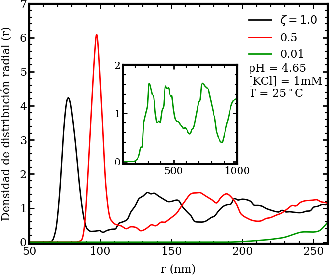
\includegraphics[width=0.45\linewidth]{Figures/graph-mc/rdf-normal.pdf}
		\caption{Densidad de distribuci\'on radial para las tres soluciones de nanogeles. Las curvas correponden a los tres factores de empaquetamiento estudiados: 1.0, 0.5 y 0.01. Las condiciones del bulk de la soluci\'on son pH 4.65, [KCl] = 1 mM y 25$^\circ$C. En el inset se muestra la curva correspondiente a $\zeta = $0.01}
		\label{fig:mc:rdf}
	\end{figure}
	
	
	\subsection{Respuesta a est\'imulos: pH, concentraci\'on salina y temperatura.}
	
	Teniendo en cuenta que las soluciones de nuestros nanogeles est\'an influenciadas por su concentraci\'on, veremos c\'omo estas soluciones influyen en su respuesta a est\'imulos, en particular los resultados que mostramos m\'as abajo surgen de los cambios en el pH, la concentraci\'on salina y la temperatura.
	
	En primera instancia veremos c\'omo se comportan las soluciones con la variaci\'on del pH.
	
	En la figura \ref{fig:mc:rvspH} se muestra el cambio del tama\~no m\'as probable, obtenido de los m\'aximos de las curvas presentadas en la figura \ref{fig:mc:densidad-probabilidad}, en funci\'on del pH de la soluci\'on. Para tal fin se han considerado tres tipos de concentraciones, o grado de empaquetamiento $\zeta = $1.0, 0.5 y 0.01.
	
	La temperatura del sistema es de 25$^\circ$C y la $[KCl]$ = 1 mM. Bajo estas condiciones solo se observa la respuesta de los segmentos de MAA.
	
	
	
	
	\begin{figure}[!htb]
		\centering
		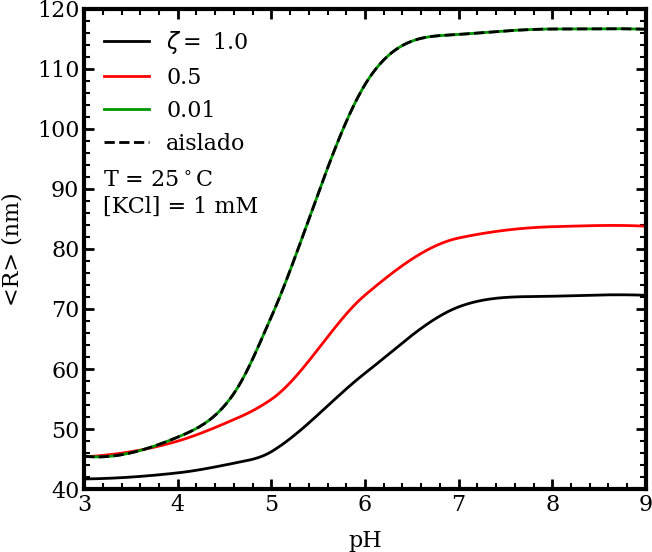
\includegraphics[width=0.45\linewidth]{Figures/graph-mc/rvspH-phis.png}
		\caption{Variaci\'on de radio medio de la soluci\'on de nanogeles en funci\'on del pH de trabajo. Temperatura 25 $^\circ$C concentraci\'on salina 1 mM en $KCl$. Cada curva correponde a un grado de empaquetamiento. En puntos el sistema aislado o dilusi\'on infinita.}
		\label{fig:mc:rvspH}
	\end{figure}
	
	
	En la figura se presentan en la curva a trazos el comportamiento de un sistema a dilusi\'on inifinita.
	Como se puede observar, el tama\~no m\'as probable de los nanogeles aumenta con el pH. Esto se debe a que el pH afecta la carga de los segmentos de MAA, que son, en parte,  responsables de la estabilidad de los nanogeles. A pH m\'as altos, los segmentos de MAA tienen adquieren una carga m\'as negativa, lo que los hace que los segmentos se repelan entre s\'i logrando expandir el nanogel.
	Este comportamiento ha sido resportado en \cite{perez2021thermodynamic}, en donde las repulsiones electrost\'aticas son disminuidas al alejar los centros de carga de la estructura del nanogel.
	
	%%%%% 
	Se puede observar que a mayor concentraci\'on, $\zeta = $1.0, el aumento de tama\~no originado por el cambio en el pH es menor respecto a las soluciones m\'as diluidas, $\zeta = $0.01.
	En soluciones m\'as concentradas, los nanogeles se encuentran m\'as cercanos entre s\'i, por lo que un aumento del radio significa una mayor interacci\'on entre ellos y, en consecuencia, un aumento en la energ\'ia del sistema.
	Tal como se observ\'o en la figura \ref{fig:mc:densidad-probabilidad}, a soluciones m\'as concentradas los nanogeles disminuyen su tama\~no para reducir las interacciones de a pares entre ellos. Este efecto es menor a pH bajos, en donde cada nanogel posee sus grupos MAA protonados (sin carga), por tanto la interacción dada por el potencial de Yukawa es cercana a cero. El grado de carga medio, $\langle f \rangle$, de las soluciones aqu\'i estudiadas se muestran en la figura \ref{fig:mc:fvspH}.
	El bajo/nulo grado de carga a pH 3 permite, a una concentraci\'on alta, $\zeta = $1.0, que las part\'iculas aumenten su tama\~no sin presentar repulsiones electrost\'aticas entre nanogeles vecinos. En consecuencia, la variaci\'on, respecto al sistema aislado, es de unos pocos nanometros. De hecho, puede notarse c\'omo a condiciones medias y bajas de $\zeta$, estos poseen el mismo valor de medio de radio($\langle R\rangle$).
	En el otro extremo, cuando el nanogel se encuentra completamente cargado (todos los segmentos de MAA desprotonados, ver figura \ref{fig:mc:fvspH}), adem\'as del potencial de Hertz, el potencial de Yukawa toma mucha relevancia. Hay una repulsi\'on entre part\'iculas cargadas con el mismo signo. El impacto de este nuevo potencial se refleja en una diferencia de m\'as de 40 nm en el radio medio de estas soluciones. Comparece $\zeta = $1.0 y 0.01.
	%%%%%%%%%%
	
	En la transici\'on de estos extremos de pH, vemos como el aumento del pH y, por tanto, el aumento de carga el\'etrica del nanogel, origina un aumento en el tama\~no. Este aumento es m\'as pronunciado a concentraciones diluidas, $\zeta = $0.01, en donde el nanogel expande su estructura para relajar las repulsiones internas con un menor costo energ\'etico por la interacci\'on con otro nanogel. En las soluciones m\'as concentradas, $\zeta = $1.0 y 0.5, el aumento de tama\~no es menor debido a la energ\'ia extra de la interacci\'on de a pares.
	Otro efecto que se observa es el desplazamiento del punto de inflexi\'on de estas curvas a valores m\'as altos de pH.
	Se asocia el punto de inflexi\'on con el pKa aparente, que se define como el pH en el cual se alcanza un $\left< f\right> = $0.5. Ver figura \ref{fig:mc:fvspH}.
	
	Las part\'iculas, en un sistema aislado, al cargarse el\'ectricamente aumentan su tama\~no para disminuir sus repulsiones internas. En las soluciones, la presencia de m\'as nanogeles pone en juego un costo energ\'etico extra al aumento de tama\~no, la interacci\'on dada por los potenciales de Hertz y Yukawa. En consecuencia, los segmentos de MAA no se desprotonan (adquieren carga positiva). Para lograr la desprotonaci\'on se requiere mayor energ\'ia para desplazar el equilibrio qu\'imico \'acido-base. Lo que se observa en un desplazamiento a mayores valores de pH.
	
	\begin{figure}
		\centering
		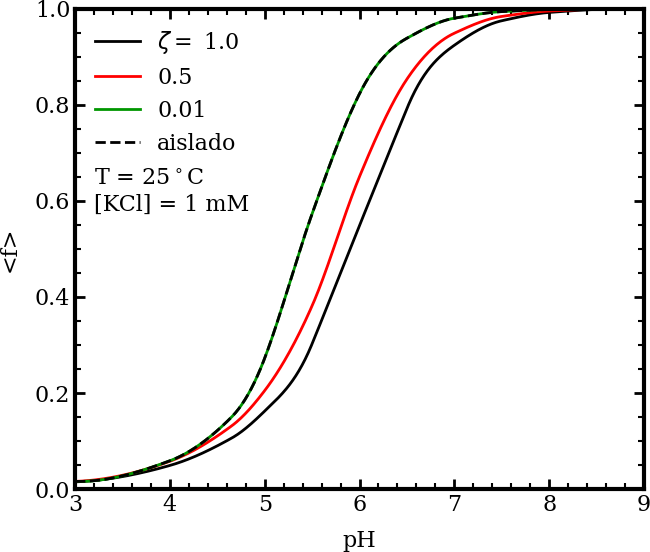
\includegraphics[width=0.45\linewidth]{Figures/graph-mc/fvspH.png}
		\caption{Grado de carga medio, $\left<f\right>$, de la soluci\'on de nanogeles en funci\'on del pH del medio. Se consideran tres densidades dadas por el factor de empaquetamiento: $\zeta =$ 1.0, 0.5 y 0.01. La temperatura del sistema es 25$^\circ$C y la concentrac\'on de sal 1 mM.}
		\label{fig:mc:fvspH}
	\end{figure}
	
	
	%%%%%
	La figura \ref{fig:mc:reentrante} muestra el tama\~no medio de las soluciones de nanogeles como funci\'on de la concentraci\'on salina. El pH es de 4.65 y la temperatura es de 25$^\circ$C. Las curvas s\'olidas corresponden a las tres factores de empaquetamiento, de trabajo: $\zeta =$ 1.0, 0.5 y 0.01. En l\'inea a trazos se incorpora el comportamiento de un nanogel aislado.
	
	Para las tres soluciones se observa una transici\'on reentrante, es decir, una respuesta no mon\'otona al aumento de la concentraci\'on salina.
	
	Este fen\'omeno se explica, en primera instancia, por los mon\'omeros cargados el\'ectricamente que componen el nanogel. La baja adsorci\'on de iones de sal, resulta en un pobre apantallamiento en repulsiones de los segmetos de MAA.En consecuencia, los nanogles aumentan su tama\~no para minimizar la energ\'ia libre qu\'imica y as\'i evitar las repulsiones. Al aumentar la concentraci\'on salina aumenta la adsorci\'on de contraiones, hay mayor apantallamiento y las repulsiones electrost\'atias son ahora de menor alcance. Esto permite una relajaci\'on en las cadenas de nanogel, observ\'andose una disminuci\'on en su radio.
	
	Nuevamente se observa un comportamiento diferente para las tres diferentes soluciones. Mayor vecindad de nanogeles, ver figura \ref{fig:mc:rdf}, hacen que interact\'uen entre ellos, aumentando la energ\'ia libre del sistema. Esta energ\'ia se incrementa a\'un m\'as si los nanogeles aumentan mucho su tama\~no, como salvoconducto para relajar sus repulsiones internas. Por lo que se observa un aumento de menor magnitud por parte de las soluciones m\'as concentradas. A medida que se diluye lo suficiente la soluci\'on, nos acercamos al comportamiento ideal, es decir, un nanogel aislado.
	
	
	
	\begin{figure}
		\centering
		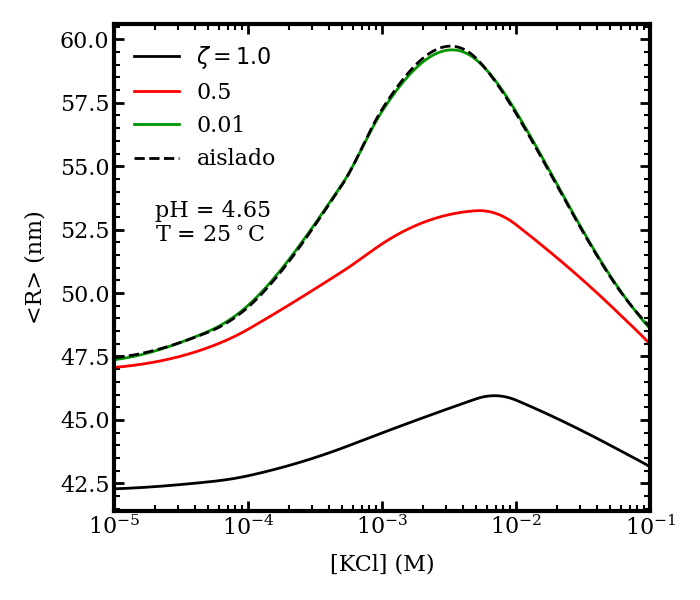
\includegraphics[width=0.45\linewidth]{Figures/graph-mc/salt-r.png}
		\caption{R medio en funci\'on de la concentraci\'on de sal, para diferentes grados en empaquetamiento.El pH de la soluci\'on es 4.65, la temperatura 25$^\circ$C, en l\'inea s\'olidas se presentan valores de  $\zeta=$ 1.0, 0.5 y 0.01, a trazos se muestra un nanogel aislado.}
		\label{fig:mc:reentrante}
	\end{figure}
	
	%%%%%
	La figura \ref{fig:mc:temperatura-r} muestra la respuesta a la temperatura de las soluciones estudiadas. Las condiciones del bulk corresponden a pH 4.65 y 1 mM [KCl], las diferentes curvas corresponden a diferentes factores de empaquetamiento: $\zeta =$  1.0 , 0.5, 0.01.
	En primera instancia, y en todos los casos,  se observa la transici\'on de un estado swelling a uno colapsado por efecto de la temperatura sobre los segmentos de NIPAm.
	Este comportamiento se debe a superar la temperatura cr\'itica de disoluci\'on (LCST) del PNIPAm. Efecto reportado en \cite{perez2021thermodynamic}.
	
	A diferencia de los resultados anteriores, en los cuales se observaba una diferencia con la concentraci\'on de la soluci\'on, no se reporta un cambio en la temperatura en la cual se da la transici\'on de un estado swelling a colapsado. 
	Al disminuir el tama\~no de cada part\'icula por efecto de la hidroficidad de los segmentos del NIPAm, tambi\'en se reducen las interacciones entre nanogeles. Este efecto es igual para cada soluci\'on, con lo cual el estado colapso es el mismo para todas ellas.
	El radio medio en el estado colapsado de las soluciones es tan bajo que no se ven efectos con la concentraci\'on en la condiciones aqu\'i mostradas. 
	
	Por otro lado a bajas temperaturas, estado swelling del gel, en donde no hay efecto alguno por parte de los segmentos de NIPAm, se obtienen tres radios medios para cada soluci\'on. El radio promedio aumenta a medida que disminuye la concentraci\'on de nanogeles. Este efecto es el reportado en la figura \ref{fig:mc:densidad-probabilidad}, en donde la mayor interacci\'on entre nanogeles para soluciones m\'as concentradas son las responsables de un menor tama\~no medio de part\'icula.
	
	
	
	\begin{figure}[!htb]
		\centering
		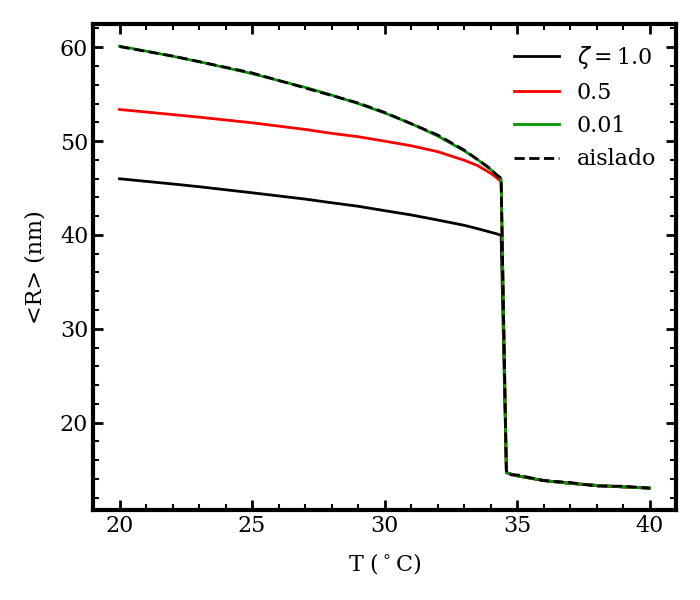
\includegraphics[width=0.45\linewidth]{Figures/graph-mc/rvst.png}
		\caption{Tama\~no medio de la soluci\'on de nanogeles como funci\'on de la temperatura del bulk. pH 4.65, $[KCl]$ 1m M y  $\zeta =$ 0.5}
		\label{fig:mc:temperatura-r}
	\end{figure}
	
	\section{Conclusiones}
	%%%%%%%%%
	En este cap\'itulo se investig\'o el comportamiento de soluciones compuestas por nanogeles polim\'ericos a diferentes grados de empaquetamiento, es decir, a diferentes concentraciones. Se desarroll\'o un modelo con el cual aplic\'o la metodolog\'ia de simulaciones Monte Carlo.
	
	El enfoque se centr\'o en la influencia de la concentraci\'on de part\'iculas sobre la respuesta a est\'imulos de nanogeles compuestos por P(NIPAM-co-MAA). Se consideraron tres est\'imulos diferentes: cambios en el pH, la temperatura y la concentraci\'on de sal. Adem\'as del efecto de la concentraci\'on de nanogeles en la soluci\'ion.
	
	Por debajo de la temperatura de transición del PNIPAm y a pH igual al pKa intr\'inseco del segmento de MAA, bajo grado de carga, se pudo observar el efecto de la concentraci\'on de nanogeles en soluci\'on.
	Los resultados obtenidos muestran que a medida que se aumenta la concentraci\'on de part\'iculas, estas disminuyen en su radio promedio. Esto se atribuye a las interacciones entre nanogeles. Para disminuir estas interacciones, cada nanogel disminuye su tama\~no.
	
	Los perfiles de las soluciones m\'as concentradas concuerdan con sistemas de fluidos l\'iquidos, mientras que para la menor concentraci\'on se obtiene un sistema que se asemeja a un gas. En consecuencia, las propiedades de esta soluci\'on se desv\'ian m\'inimamente del sistema a diluci\'on infinita.
	La disminuci\'on del  tama\~no para minimizar las interacciones entre part\'iculas es el responsable de los cambios en la respuesta a los est\'imulos de pH, temperatura y concentraci\'on de sal. El comportamiento es cualitativamente similar a un sistema con diluci\'on infinita, pero de menor magnitud.
	
	En particular, la respuesta a cambios de pH tambi\'en conlleva un aumento en el pKa aparente de la soluci\'on. Par\'ametro importante al momento de caracterizar una soluci\'on.
	Otra particularidad que se mostr\'o es el efecto de la temperatura.
	A diferencia de observar un cambio en la temperatura de transici\'on, del mismo modo que del pKa aparente de las soluciones, se encontr\'o que las tres soluciones estudiadas conflu\'ian a un mismo radio medio y a una misma temperatura de transici\'on. Los nanogeles en estado colapsado no logran interactuar con otras part\'iculas vecinas, en consecuencia no hay efecto del grado de empaquetamiento en estas condiciones.
	
	